\documentclass{article}
\usepackage{tikz}

% Load required TikZ libraries for extra shapes
\usetikzlibrary{shapes.geometric, shapes.misc}

\begin{document}

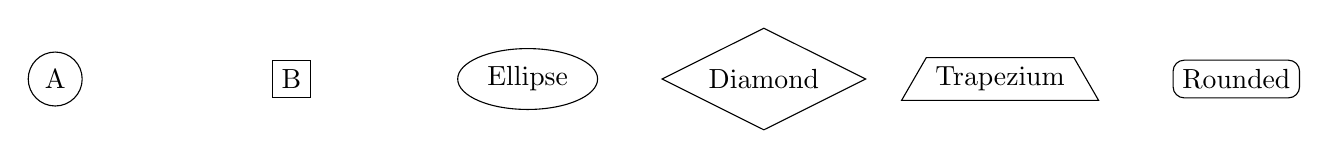
\begin{tikzpicture}[scale=1]

  % --- Circle node ---
  \node[draw, circle] at (0,0) {A};

  % --- Rectangle node ---
  \node[draw, rectangle] at (3,0) {B};

  % --- Ellipse node ---
  \node[draw, ellipse] at (6,0) {Ellipse};

  % --- Diamond node (requires shapes.geometric library) ---
  \node[draw, diamond, aspect=2] at (9,0) {Diamond};

  % --- Trapezoid node (requires shapes.geometric library) ---
  \node[draw, trapezium, trapezium stretches] at (12,0) {Trapezium};

  % --- Rounded rectangle node (requires shapes.misc library) ---
  \node[draw, rectangle, rounded corners] at (15,0) {Rounded};

\end{tikzpicture}

\end{document}
